\documentclass[titlepage,a4paper]{article}
\usepackage[T1]{fontenc}		% font encode
\usepackage[utf8]{inputenc}	 % input encode
\usepackage[english]{babel}		% secondary and main languages
\usepackage{authblk}			% to add affiliation
\usepackage[tt]{titlepic}		% to add the logo in first page
\usepackage{graphicx}			% to add images
\usepackage{gensymb}			% used for symbols as °(\degree)
\usepackage{amsmath}
\usepackage{mathtools}			% used for math formulae
\usepackage{float}
\usepackage{titlesec}			%used to add \sectionbreak command
\usepackage{appendix}
\usepackage{hyperref}
\usepackage{footnote}
\usepackage{enumitem}
\usepackage{blindtext}
\usepackage{graphicx}
\usepackage{caption}
\usepackage{subcaption}
\usepackage{listings}
\usepackage{xcolor}
\usepackage{hyperref}
\usepackage{rotating}
\usepackage{siunitx}
\usepackage{listings}		%code listings (lstlisting)
\usepackage{color}

\setlistdepth{9}									% enumerate depth 
\newlist{req_enum}{enumerate}{9}					% definition of a new enumerate type
\setlist[req_enum]{label=\thesubsection.\arabic{*}.}	% include the chapter number

\definecolor{gray}{rgb}{0.4,0.4,0.4}
\definecolor{darkblue}{rgb}{0.0,0.0,0.6}
\definecolor{cyan}{rgb}{0.0,0.6,0.6}

\lstset{basicstyle=\ttfamily,columns=fullflexible,showstringspaces=false,tabsize=2}

\lstdefinestyle{custompython}{backgroundcolor=\color{white},belowcaptionskip=1\baselineskip,breaklines=true,frame=L,xleftmargin=\parindent,language=Python,showstringspaces=false,basicstyle=\footnotesize\ttfamily,keywordstyle=\bfseries\color{darkblue},commentstyle=\itshape\color{green!40!black},identifierstyle=\color{blue},stringstyle=\color{orange},
}


\lstdefinestyle{custombash}{basicstyle=\color{white},backgroundcolor=\color{black},belowcaptionskip=1\baselineskip,breaklines=true,frame=L,xleftmargin=\parindent,language=bash,showstringspaces=false,morekeywords={roslaunch,rosrun},basicstyle=\footnotesize\ttfamily,keywordstyle=\bfseries\color{yellow},commentstyle=\itshape\color{green},identifierstyle=\color{white},stringstyle=\color{orange},
}


\lstdefinelanguage{XML}{morestring=[b]", morestring=[s]{>}{<}, stringstyle=\color{red}, identifierstyle=\color{darkblue}, commentstyle=\color{green}, keywordstyle=\color{cyan}, morekeywords={name,xmlns,version,type}% list your attributes here
}

\newcommand{\sectionbreak}{\clearpage}	%to start new section in a new page

\graphicspath{{img/}{img/Johnny/}{img/rob/screenshots/}}

\renewcommand\Authfont{\fontsize{12}{14.4}\selectfont}
\renewcommand\Affilfont{\fontsize{10}{10.8}\selectfont}

%intestazione
\title{
\includegraphics[width=4cm, keepaspectratio]{unipi_blu}\hspace{2cm}
\includegraphics [width=4cm, keepaspectratio]{santanna}~\\[2cm]
\textbf{\LARGE Design of Embedded Systems}\\[1cm] ESSTA, Energy Saving Smart-home distributed Temperature control Application}

\author{\emph{Falzone Giovanni}}
\affil{\emph{jointly M.Sc Embedded Computing Systems}}
\affil{\emph{Sant'Anna School of Advanced Studies}}
\affil{\emph{University of Pisa}}

\begin{document}
\maketitle
\tableofcontents

\newpage
\section{Introduction}
The purpose of this project is to realize a smart-home application to control the heating system of a building based on the temperature of each room, in order to minimize the consumption of the building each room apply an energy saving function reducing the desired temperature when it is not needed.
The system is composed by two differ modules
\begin{itemize}
	\item central unit module 
	\item room module
\end{itemize}

\subsection{Central Unit}
The \textit{Central Unit} has the role of coordinator that retrieve the status of each room and computes the average values for the building.\\

\subsubsection{Graphical user interface}
Using a graphical User Interface the module represents the average values of the building and the values for each room, the graphical User Interface is composed by:
\begin{itemize}
	\item \textit{Main page} to represent the overview of the building
	\item \textit{Room page} to represent the status of each room
	\item \textit{Settings page} to set the desired temperature
\end{itemize}

Whenever the \textit{Main page} is selected the module shall represent the average values among all the rooms for \textit{Temperature}, \textit{Humidity} and \textit{Usage}.\\
Whenever the \textit{Main page} is selected the module shall represent the \textit{Energy Saving} if at least one room is set to \textbf{Energy Saving mode}.\\
Whenever the \textit{Main page} is selected the module shall represent the \textit{Warning} if at least one room is set to \textbf{crashed}.\\
Whenever the \textit{Main page} is selected the module shall allow the user to move in the \textit{Settings page}, next and previous \textit{Room page}.\\

Whenever the \textit{Settings page} is selected the module shall represent the \textit{Desired Temperature} and shall allow the user to increase or deacrease it by a factor of 0.5 C\degree in the range of 15 C\degree and 30 C\degree.\\
Whenever the \textit{Settings page} is selected the module shall represent the average values among all the rooms for \textit{Humidity} and \textit{Usage}.\\
Whenever the \textit{Settings page} is selected the module shall represent the \textit{Energy Saving} if at least one room is set to \textbf{Energy Saving mode}.\\
Whenever the \textit{Settings page} is selected the module shall represent the \textit{Warning} if at least one room is set to \textbf{crashed}.\\
Whenever the \textit{Settings page} is selected the module shall allow the user to move in the \textit{Main page}.\\

Whenever the \textit{Room page} is selected the module shall represent the average values among all the rooms for \textit{Temperature}, \textit{Humidity} and \textit{Usage}.\\
Whenever the \textit{Room page} is selected the module shall represent the \textit{Energy Saving} if at least one room is set to \textit{Energy Saving mode}.\\
Whenever the \textit{Room page} is selected the module shall represent the \textit{Warning} if at least one room is set to \textbf{crashed}.\\
Whenever the \textit{Room page} is selected the module shall allow the user to move in the \textit{Main page}, \textit{Settings page}, next and previous \textit{Room page}.\\

The graphical user interface shall represent the following information as reported in the table \ref{tab:GraphicalInformations}.
\begin{table}[H]
	\centering
			\begin{tabular}{||l | l||} 
			\hline
			\textbf{Information}	& \textbf{Format} \\ 
			\hline
			Temperature	& C\degree \\ 
			\hline
			Humidity	& \% \\ 
			\hline
			Usage		& \% \\ 
			\hline
			Energy Saving	& boolean \\ 
			\hline
			Warning		& boolean \\ 
			\hline
		\end{tabular}
		\captionof{table}{Display Information\label{tab:GraphicalInformations}}
\end{table}

\subsubsection{Communication}
Whenever a \textit{Room Request message} is sent and the \textit{Room Status message} is not received within 20s the module shall mark the room as \textbf{crashed}.
The module shall send the \textit{Room Request message} for each room at least every 30s.

%--------------------------------------
\subsection{Room Module}
The purpose of this module is to control the temperature of the room acting on a valve in order to 
reach and maintain the \textit{GoalTemperature}.

\subsubsection{Energy Saving mode}
In order to minimize the consumption the module keep tracks of the presence of motion inside the room
using a motion sensor. \\

If a motion is detected in the last 30s, the module shall set the \textit{GoalTemperature} to the one set by the user,otherwise the module shall set the \textit{GoalTemperature} to:

\begin{equation}
	GoalTemperature = DesiredTemperature - EnergySavingTemperatureOffset
\end{equation}
Whenever the module is in \textit{Energy Saving mode} it shall notify it through the \textit{Interface}.

\subsubsection{Valve control}
In order to control the heating of the room the valve is moved to different positions based on the temperature error 
(\textit{ActualTemperature} - \textit{GoalThemperature}) as in the following table, 
whenever one of these rules is valid the module shall move the valve in the correspondent position described in the third column of the table \ref{tab:ValvePositions} as percentage of maximum flow.
\begin{center}
	\begin{tabular}{| l | l | l |} 
		\hline
		\textbf{rule} & \textbf{valve position} & \textbf{Flow in \%}\\
		\hline
		\begin{math} error < -HIGH \end{math} &  OPEN\_POSITION & 100\\
		\hline
		\begin{math} error \in [-HIGH, -APPROCHING) \end{math}  & HIGH\_POSITION & 75\\
		\hline
		\begin{math} error \in [-APPROCHING, +APPROCHING] \end{math} & MIDDLE\_POSITION & 50 \\
		\hline
		\begin{math} error \in (APPROCHING, HIGH] \end{math} & LOW\_POSITION & 25\\
		\hline
		error > HIGH &  CLOSED\_POSITION & 0 \\
		\hline
	\end{tabular}
	\captionof{table}{\label{tab:ValvePositions}}
\end{center}
Whenever the valve is in \textit{OPEN\_POSITION} or \textit{CLOSED\_POSITION} the module shall check the position and set \textbf{Valve Error} if it is not valid.

In the following table\ref{tab:TemperatureThresholds} are reported the temperature thresholds:
\begin{center}
	\begin{tabular}{||l | l||} 
		\hline
		HIGH 		& 2 C\degree \\ 
		\hline
		APPROCHING 	& 1 C\degree \\ 
		\hline
	\end{tabular}
	\captionof{table}{\label{tab:TemperatureThresholds}}
\end{center}


\subsubsection{Communication}
Whenever a \textit{Room Request message} is not received within 60s the module shall send the \textit{Room Status Message} and set the \textbf{Communication error}.

\subsubsection{Errors}
Whenever one of the errors are set, the module shall notify it through the \textit{Interface}.
In the following table \ref{tab:RoomErrors} are reported the possible errors.
\begin{center}
	\begin{tabular}{|| l ||} 
		\hline
		\textbf{Valve error} \\ 
		\hline
		\textbf{Communication error} \\ 
		\hline
		\textbf{Sensor error} \\ 
		\hline
	\end{tabular}
	\captionof{table}{\label{tab:RoomErrors}}
\end{center}

\section{Room Module}
The aim of this module is to control the temperature of the room and act on the valve in order to 
achieve the desired temperature set by the user through the \textit{Central Unit} but minimizing the consumption
reducing the desired temperature when the room is not used.
\newline
The module is composed by:
\begin{itemize}
	\item Temperature sensor
	\item Humidity sensor
	\item Motion sensor
	\item Valve actuator
	\item Wireless communication module
	\item Error led
	\item Eco mode led
	\item Motion detection led
\end{itemize}

\subsection{Temperature control}
The module adjust the temperature of the room acting on a valve.
The valve is set to different positions based on the temperature error (difference between the actual temperature and the desired themperature):
\begin{itemize}
	\item if the temperature error is below then -COLD\_THRESHOLD the valve is moved in OPEN\_POSITION
	\item if the temperature error is below then -WARM\_THRESHOLD the valve is moved in HIGH\_POSITION
	\item if the temperature error is between a [-APPROCHING\_THRESHOLD, APPROCHING\_THRESHOLD] the valve is moved in HALF\_POSITION
	\item if the temperature error is greater then WARM\_THRESHOLD the valve is moved in LOW\_POSITION
	\item if the temperature error is greater then HOT\_THRESHOLD the valve is moved in CLOSED\_POSITION
\end{itemize}

\subsection{Energy Saving mode}
In order to minimize the consumpion the module keep tracks oF the presence of motion inside the room
using a motion sensor.
If a predefined number of motion is detected in a time slot, the module set the desired temperature to the one set by the user.
If there is the number of motions counted is greater then a predefined thresholf the module set the desired temperature 
to a value equal to the user desired temperature minus a default value ENERGY\_SAVING\_TEMPERATURE\_DIFFERENCE.

\newpage
\subsection{User Requirements}
\begin{req_enum}
	\item Whenever a motion is not detected the module shall move in Eco mode
	\item Whenever difference between the actual temperature and the desired temperature is included in the range 
	[-APPROACHING\_THRESHOLD, APPROACHING\_THRESHOLD] the valve shall be in HALF\_POSITION
\end{req_enum}

\subsection{Functional requirements}
\begin{req_enum}
	\item \textbf{Initialization}
	\begin{req_enum}[label*=\arabic*.]
		\item Whenever the module is turn on it shall send an initialization message to the \textit{Central Unit} and wait for the response
		\item During the initialization phase the module shall continue blinking the ERROR\_LED
		\item During the initialization phase the module shall check the valve moving it from the CLOSED\_POSITION to the OPEN\_POSITION
		\item During the initialization phase the module shall check the temperature sensor until a correct value is received
		\item During the initialization phase the module shall check the humidity sensor until a correct value is received
	\end{req_enum}

	\item \textbf{Communication}
	\begin{req_enum}[label*=\arabic*.]
		\item The module shall move in COMMUNICATION\_ERROR status if does not receive the check message from the \textit{Central Unit} within 1 minute
		\item The module shall send its status to the \textit{Central Unit} every 10 seconds
		\item The module shall send its status in conformance with JSON format
		\begin{req_enum}[label*=\arabic*.]
			\item The status message shall include its ID in the status message
			\item The status message shall include the Eco mode status
			\item The status message shall include its sensors list
			\item The status message shall include its actuators list
			\item The status message shall include the name of every sensor and actuator
			\item The status message shall include the format for every numerical value
		\end{req_enum}
		\item Whenever a check message from the \textit{Central Unit} is not received whitin 1 minute the module shall go in COMMUNICATION\_ERROR
	\end{req_enum}

	\item \textbf{Valve management}
	\begin{req_enum}[label*=\arabic*.]
		\item The module shall change the position of the valve every 30 seconds
		\item The valve shall be in one of the allowed positions
		\begin{req_enum}[label*=\arabic*.]
			\item The valve shall be in OPEN\_POSITION whenever the difference between the actual temperature and the desired temperature is below -COLD\_THRESHOLD C\degree
			\item The valve shall be in HIGH\_POSITION whenever the difference between the actual temperature and the desired temperature is greater then -COLD\_THRESHOLD C\degree and below -APPROACHING\_THRESHOLD C\degree
			\item The valve shall be in HALF\_POSITION whenever the difference between the actual temperature and the desired temperature is greater or equal then -APPROACHING\_THRESHOLD C\degree and below or equal then APPROACHING\_THRESHOLD C\degree
			\item The valve shall be in LOW\_POSITION whenever the difference between the actual temperature and the desired temperature is greater then APPROACHING\_THRESHOLD C\degree and below or equal then HOT\_THRESHOLD C\degree
			\item The valve shall be in CLOSED\_POSITION whenever the difference between the actual temperature and the desired temperature is greater then HOT\_TEMP C\degree
		\end{req_enum}
	\end{req_enum}

	\item \textbf{Sensors management}
		\begin{req_enum}[label*=\arabic*.]
			\item The module shall update the actual temperature every 10 seconds
			\item Whenever the actual temperature is below 15 C\degree or greater then 40 C\degree the module shall go in temperature error state
			\item The module shall update the actual humidity every 10 seconds
			\item The module shall update the presence of motion every 5 seconds
			\item Whenever a motion is detected the module shall notify it turning on the MOTION\_LED
			\item Whenever a motion is detected the module shall increase a MOTION\_COUNTER value
			\item Whenever a motion is not detected and the MOTION\_COUNTER is greater then zero the module shall decrease the MOTION\_COUNTER
		\end{req_enum}

	\item \textbf{Energy Saving management}
		\begin{req_enum}[label*=\arabic*.]
			\item Whenever the MOTION\_COUNTER reaches the MOTION\_THRESOLD value the module shall move in normal mode
			\item Whenever the MOTION\_COUNTER is below the MOTION\_THRESOLD value the module shall move in Eco mode
			\item Whenever the module is in Eco mode the module shall notify it turning on the ECO\_MODE\_LED
			\item Whenever the module is in Eco mode the module shall set the desired temperature with the difference between the desired temperature and the ENERGY\_SAVING\_TEMPERATURE\_DIFFERENCE
		\end{req_enum}

		\item \textbf{Error handling}
		\begin{req_enum}[label*=\arabic*.]
			\item Whenever an error case is achieved the module shall notify the precense of errors turning on the ERROR\_LED
			\item Whenever an error case is achieved the module shall continue sending a status message with the error field set to 1 to the \textit{Central Unit}
		\end{req_enum}

\end{req_enum}

\section{Central Unit}
\section{SySML Functional model}
In the figure \ref{fig:SystemComponents} is reported the functional Block Definition Diagram that describes the composition of the system, composed by one Central Unit and up to eight Rooms, the two modules are connected via two FlowPort as shown in \ref{fig:SystemInternals}.
The Central Unit send a \textit{RoomRequest} message composed as follows:
\begin{center}
	\begin{tabular}{||l | l| l ||} 
		\hline
		\textbf{parameter} 	& \textbf{type} & \textbf{[Min,Max]}\\ 
		\hline
		Id 					&  Natural & [1,8] \\ 
		\hline
		DesiredTemperature 	&  Float & [15.00, 30.00] \\ 
		\hline
	\end{tabular}
	\captionof{table}{Room Request variables \label{tab:RoomRequest}}
\end{center}
The Room module send a \textit{RoomStatus} message composed as follow:
\begin{center}
	\begin{tabular}{||l | l| l ||} 
		\hline
		\textbf{parameter} 	& \textbf{type} & \textbf{[Min,Max]}\\ 
		\hline
		Id 					&  Integer & [1,8] \\ 
		\hline
		Eco				 	&  Boolean & [0, 1] \\ 
		\hline
		Temperature			&  Float & [15.00, 30.00] \\ 
		\hline
		Humidity			&  Float & [0.00, 100.00] \\ 
		\hline
		Valve				&  Integer & [0, 100] \\ 
		\hline
	\end{tabular}
	\captionof{table}{Room Status variables \label{tab:RoomStatus}}
\end{center}

\begin{figure}[H]
	\centering
	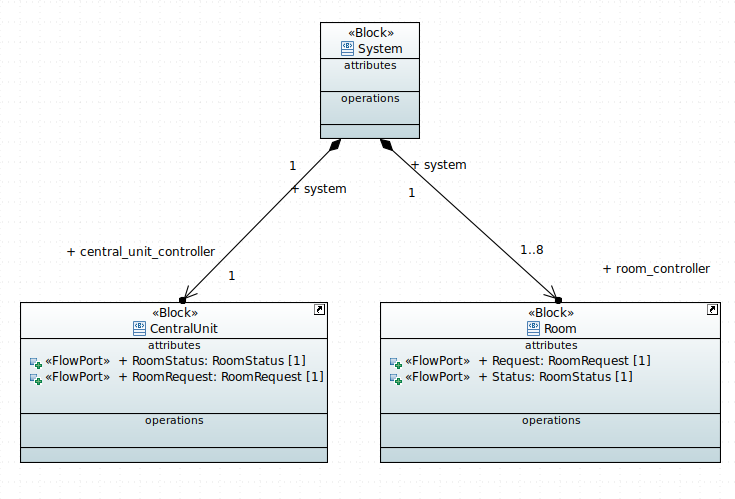
\includegraphics[width=12cm,keepaspectratio]{img/sysml/SystemComponents}
	\caption{System Components}
	\label{fig:SystemComponents}
\end{figure}
\begin{figure}[H]
	\centering
	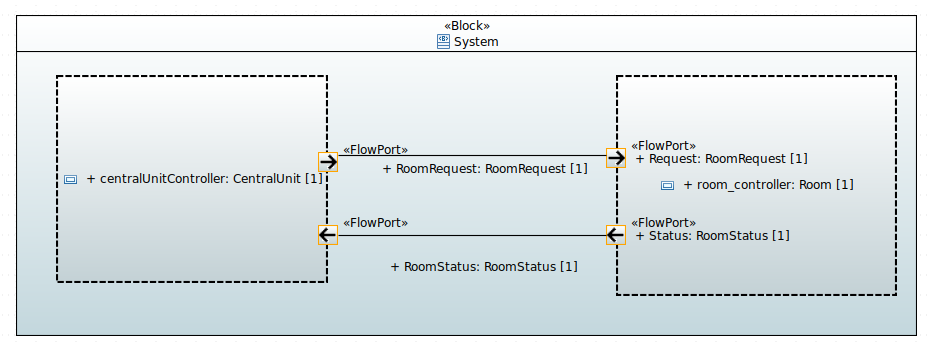
\includegraphics[width=12cm,keepaspectratio]{img/sysml/SystemInternals}
	\caption{System Internals}
	\label{fig:SystemInternals}
\end{figure}

\subsection{Central Unit}
The \textit{Central Unit} is composed by two modules, the \textit{RoomsManager} and the \textit{UserInterfaceManager}.
The \textit{RoomsManager} implements the functionalities related to the status of each room.
The \textit{UserInterfaceManager} that implements the functionalities related to represent the status of the system.
The two components exchange data as shown in \ref{fig:CentralUnit_internals}.
\begin{figure}[H]
	\centering
	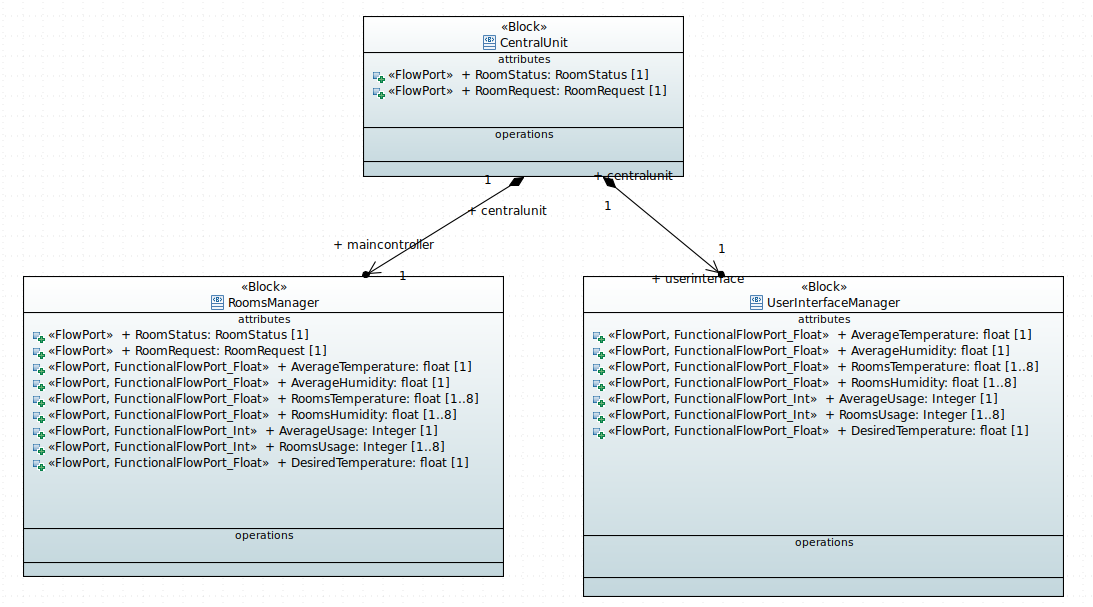
\includegraphics[width=12cm,keepaspectratio]{img/sysml/CentralUnitComponents}
	\caption{Central Unit components}
	\label{fig:CentralUnit_components}
\end{figure}

\begin{figure}[H]
	\centering
	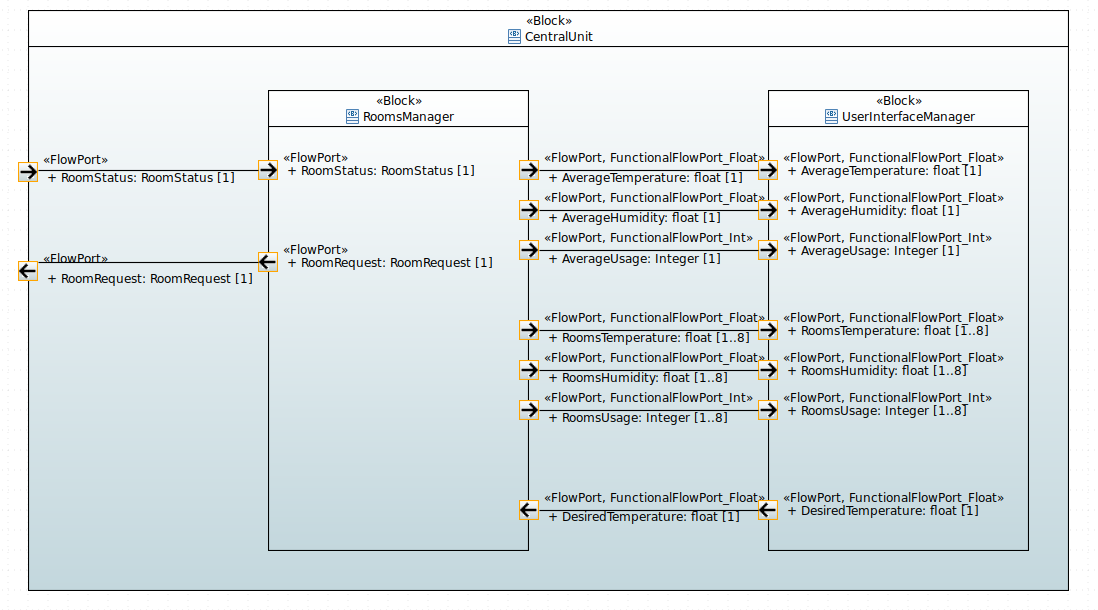
\includegraphics[width=12cm,keepaspectratio]{img/sysml/CentralUnitInternals}
	\caption{Central Unit internals}
	\label{fig:CentralUnit_internals}
\end{figure}

\subsection{Room module}
The main component of this module is the \textit{MainController} composed by different functions as shown in \ref{fig:RoomInternals}.
\begin{figure}[H]
	\centering
	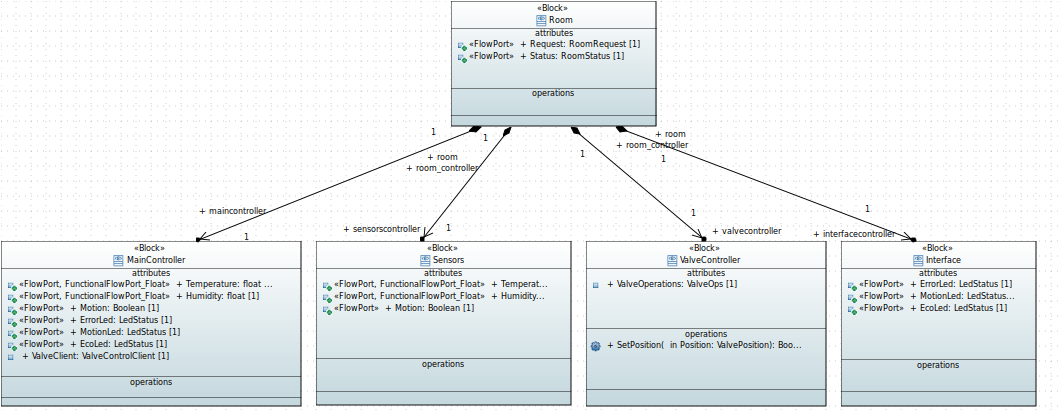
\includegraphics[width=13cm,keepaspectratio]{img/sysml/RoomComponents}
	\caption{Room Components}
	\label{fig:RoomComponents}
\end{figure}

\begin{figure}[H]
	\centering
	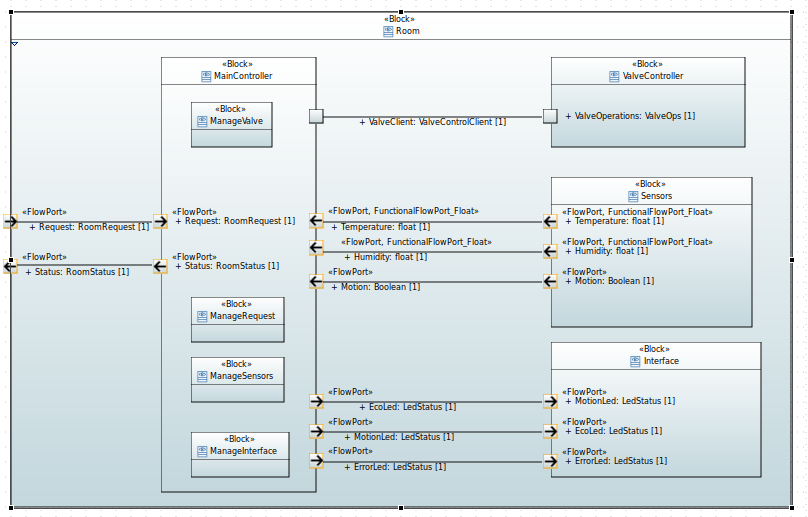
\includegraphics[width=13cm,keepaspectratio]{img/sysml/RoomInternals}
	\caption{Room Internals}
	\label{fig:RoomInternals}
\end{figure}

\begin{figure}[H]
	\centering
	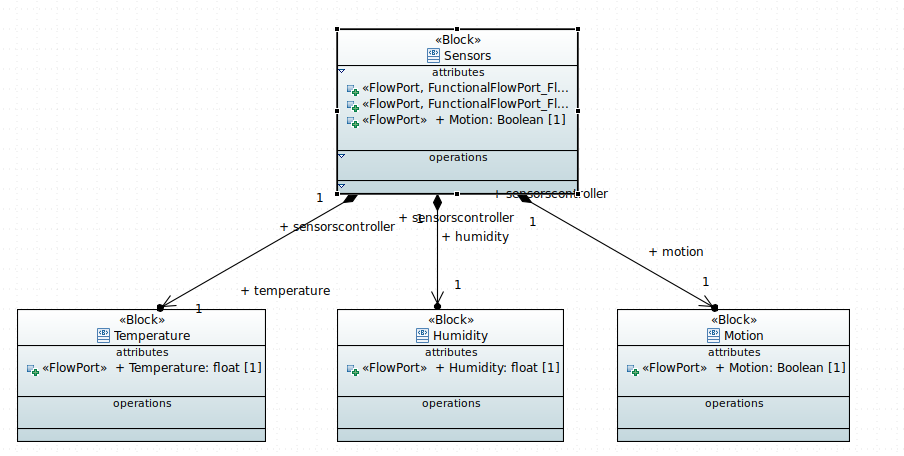
\includegraphics[width=13cm,keepaspectratio]{img/sysml/SensorsComponents}
	\caption{Room sensors components}
	\label{fig:room_sensors_components}
\end{figure}

\begin{figure}[H]
	\centering
	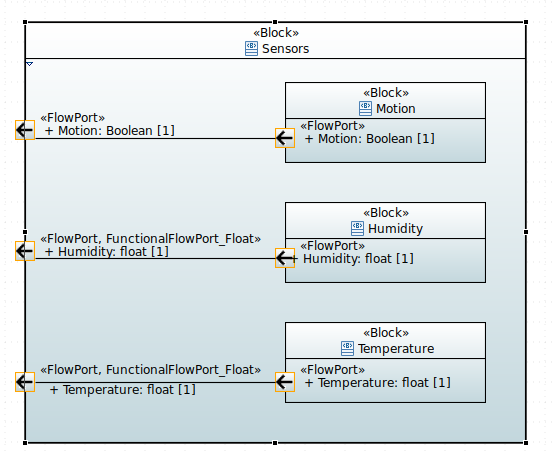
\includegraphics[width=8cm,keepaspectratio]{img/sysml/SensorsInternals}
	\caption{Room sensors internals}
	\label{fig:room_sensors_internals}
\end{figure}

\begin{figure}[H]
	\centering
	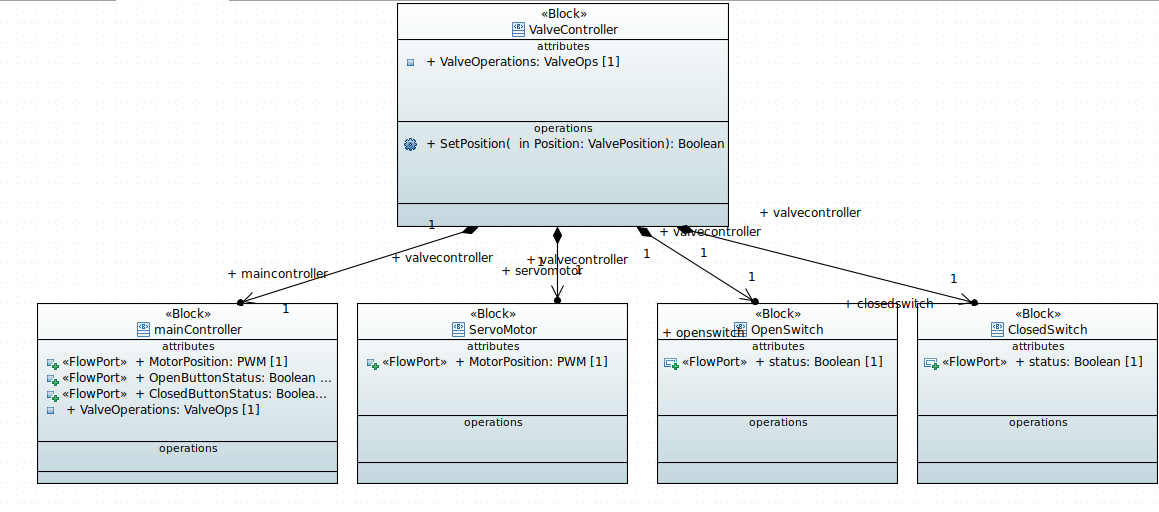
\includegraphics[width=12cm,keepaspectratio]{img/sysml/ValveControllerComponents}
	\caption{Valve Controller components}
	\label{fig:valve_dbd}
\end{figure}

\begin{figure}[H]
	\centering
	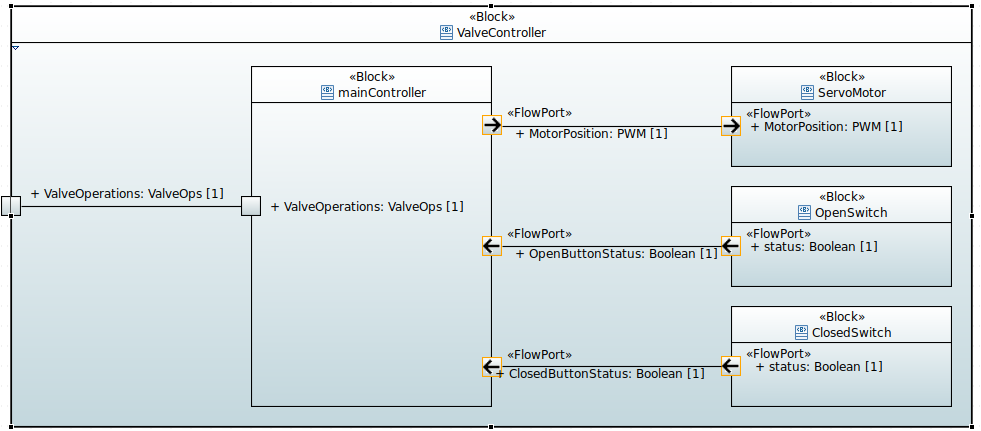
\includegraphics[width=12cm,keepaspectratio]{img/sysml/ValveControllerInternals}
	\caption{Valve Controller internals}
	\label{fig:valve_internals}
\end{figure}

\subsection{Communication State Machines}
In the following pictures are illustrated the behaviour of the communication between the \textit{CentralUnit} and the \textit{Room}.

\begin{figure}[H]
	\centering
	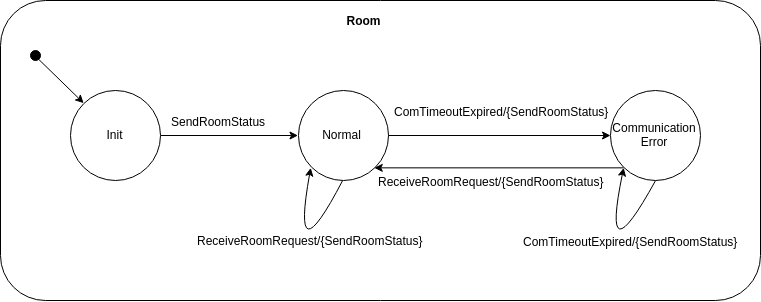
\includegraphics[width=12cm,keepaspectratio]{img/Com_SM_Room}
	\caption{Room communication management}
	\label{fig:room_com}
\end{figure}

In the figure \ref{fig:CU_com_receiver} is described the behaviour of the receiver part in the \textit{CentralUnit}, for readibility is reported just the case of a paramentric room X.\\

In the figure \ref{fig:CU_com_sender} is described the behaviour of the sender part in the \textit{CentralUnit}, for readibility is reported just the case of 2 rooms.

\begin{figure}[H]
	\centering
	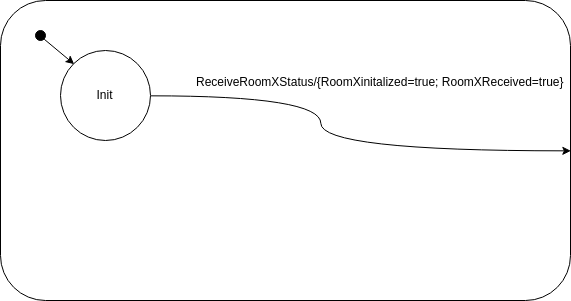
\includegraphics[width=10cm,keepaspectratio]{img/Com_SM_CU_Receiver}
	\caption{Central Unit communication receiver management}
	\label{fig:CU_com_receiver}
\end{figure}

\begin{figure}[H]
	\centering
	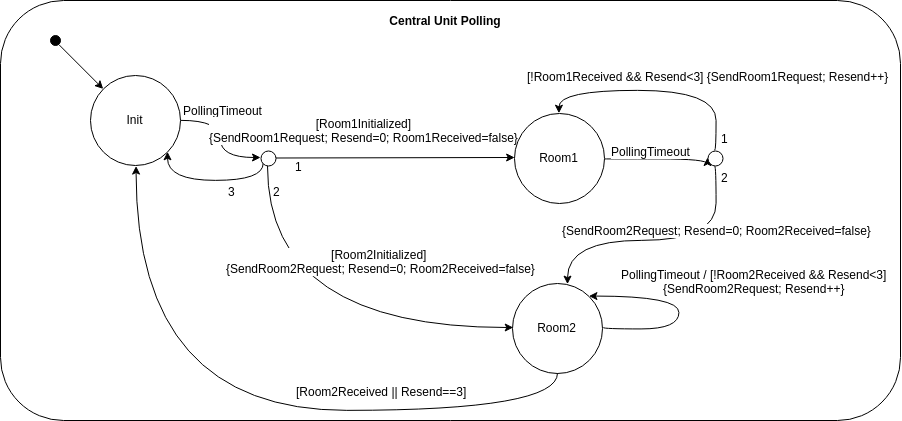
\includegraphics[width=12cm,keepaspectratio]{img/Com_SM_CU_Sender}
	\caption{Central Unit communication sender management}
	\label{fig:CU_com_sender}
\end{figure}

\section{Implementation, Central Unit module}
\begin{figure}[H]
	\centering
	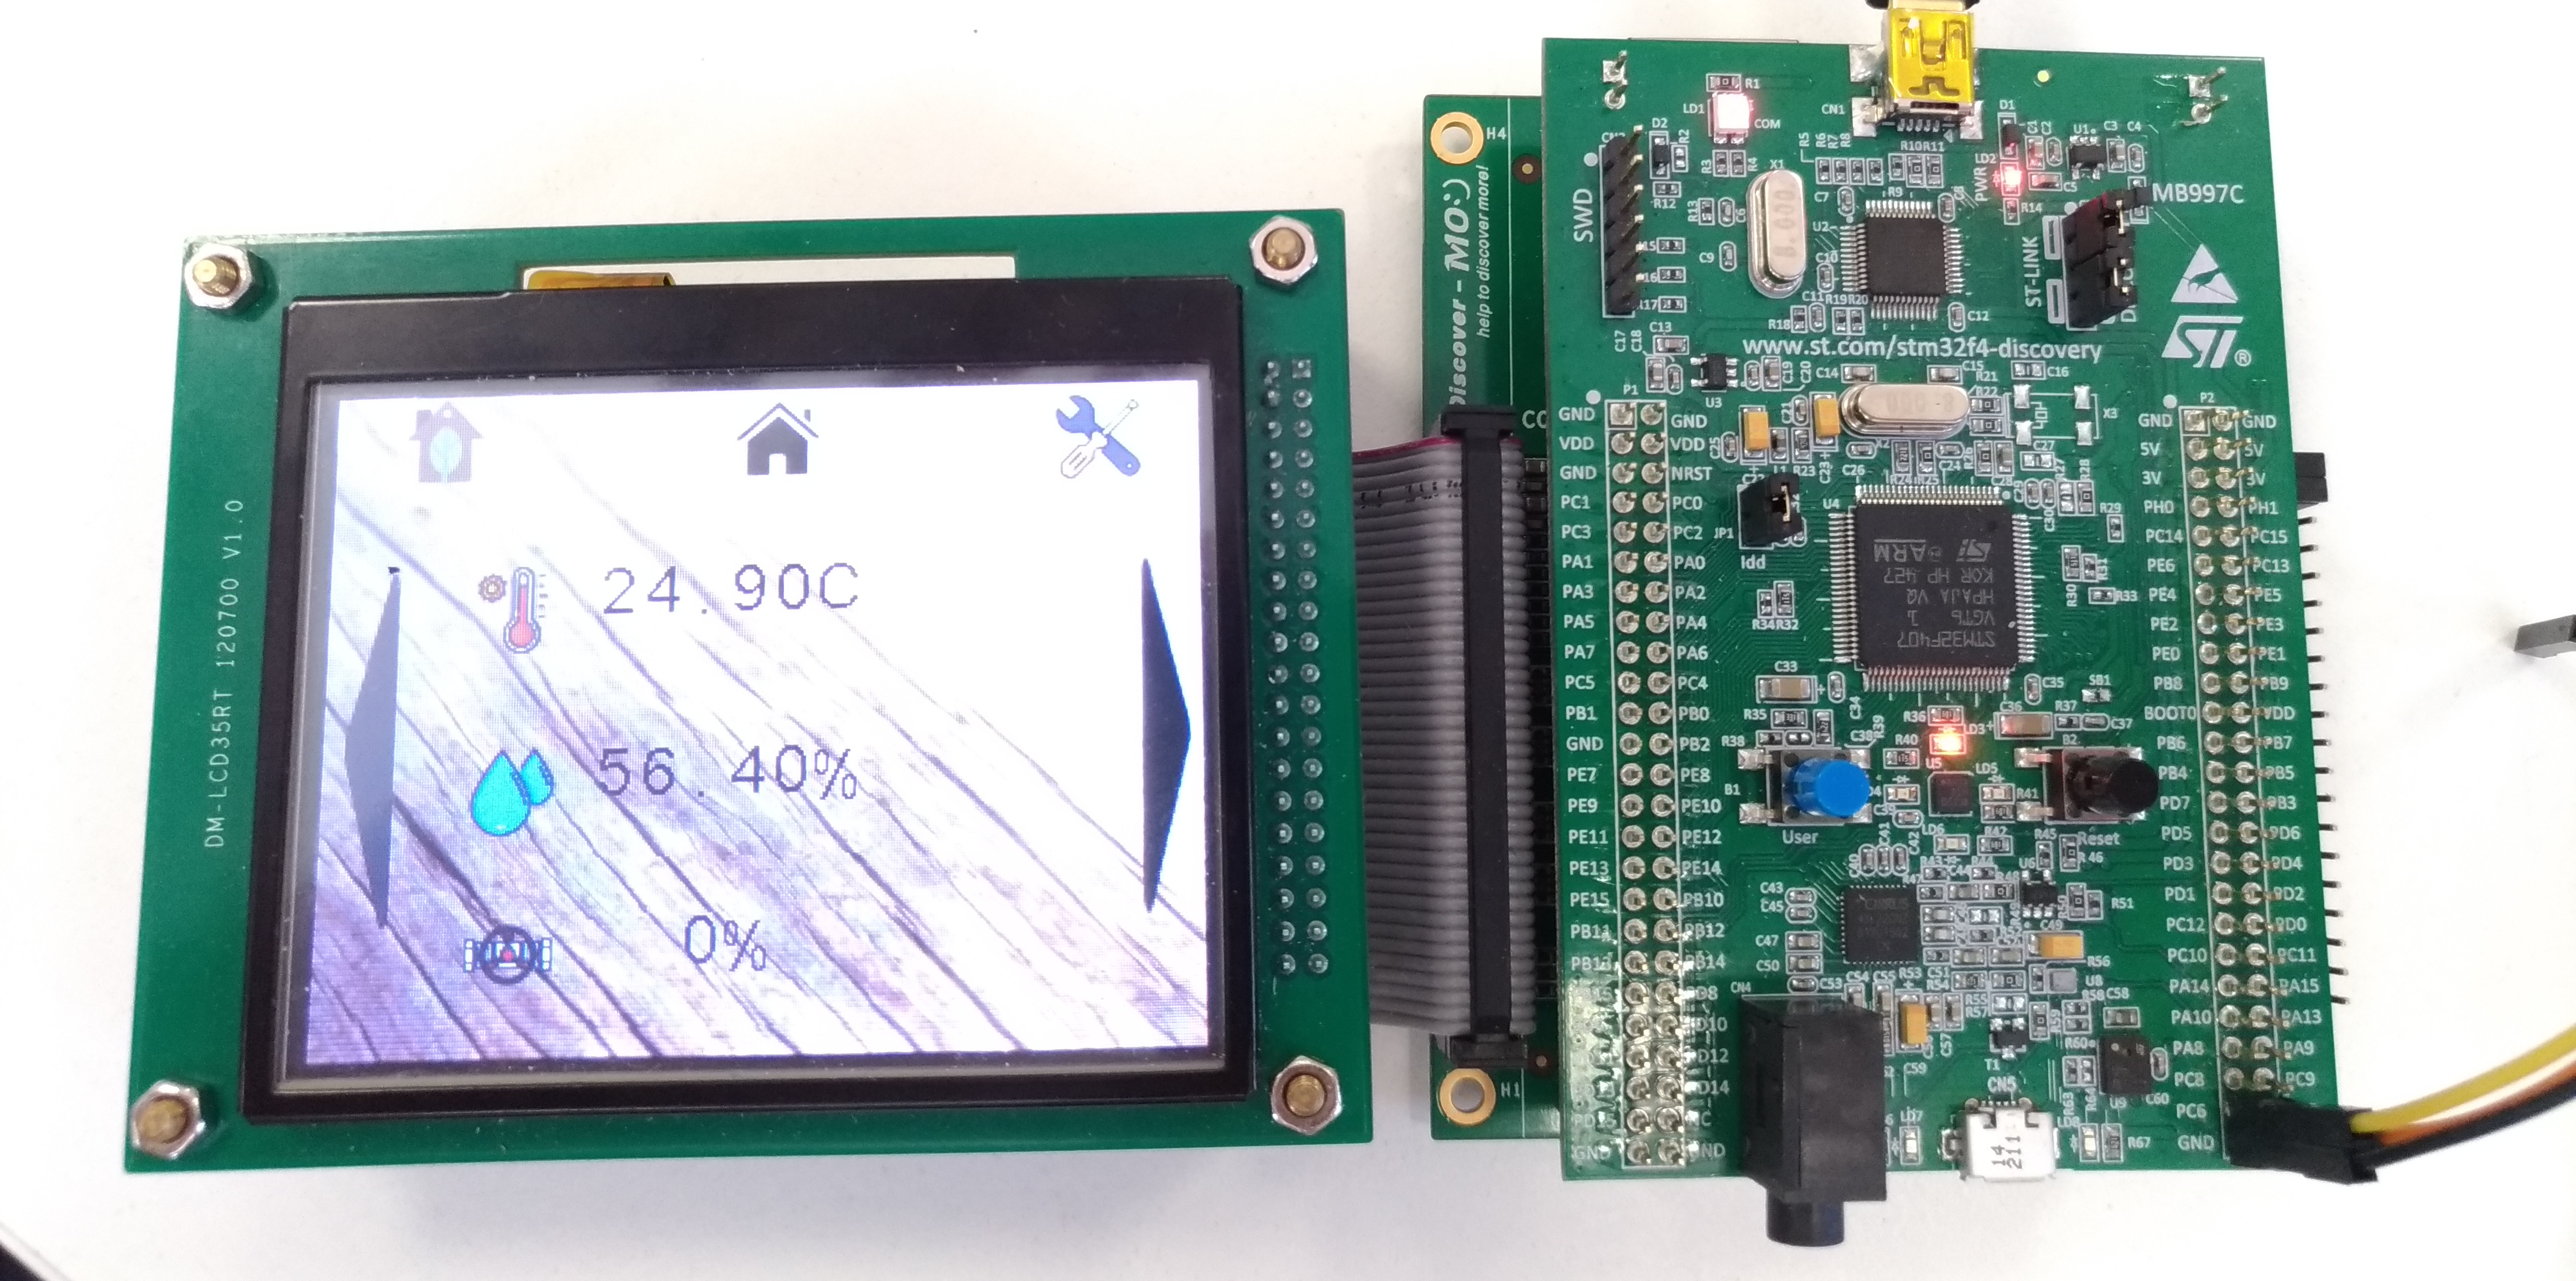
\includegraphics[width=8cm,keepaspectratio]{img/CentralUnit}
	\caption{Central Unit module}
	\label{fig:CentralUnit}
\end{figure}

The module is composed by:
\begin{itemize}
	\item STM32F407VG DISCOVERY powered by ARM Cortex-M4 32-bit
	\item LCD board Touchscreen 3”5
\end{itemize}
In the discovery board are running the \textit{Central Unit's} tasks on top of Erika RTOS, the system is composed by three different tasks reported in the table \ref{tab:CU_Tasks}.\\
Whenever a \textit{Room Status} message arrives through the \textit{USART} interface, the \textit{Check message} aperiodic task is activated in order to check the message and execute the \textit{Room's} functionalities.\\
The \textit{Check  message} task apply a simple JSON compliance test and check each field name and value of the message, then the message is converted in a \textit{Room structure} and the Room's status and \textit{Building} status are updated.\\
While the \textit{Check message} task has the role of processing the incoming \textit{Room Status}, the \textit{Polling} task has the role of managing the rooms sending a check message periodically one room after the other, 
if the response \textit{Room Status} message doesn't arrive within the next task's job it's considered as an error and the same \textit{Room Request} message is sent until a maximum of 3 resend, then the room is marked as crashed.\\
The \textit{Graphic} task has the role to represent the data of the building and for each room depending on the selected page by the user, in the settings page the user is able to set the desired temperature that will be sent starting from the next job of the \textit{Polling} task.\\
\begin{center}
	\begin{tabular}{||c | c | c ||} 
		\hline
		Name 	& Frequency & Priority	\\ 
		\hline
		\textbf{Check message task}	&	Aperiodic		& 3 	\\ 
		\hline
		\textbf{Polling task}		&	0.2Hz			& 2 	\\ 
		\hline
		\textbf{Graphic task}		&	10Hz			& 1 	\\ 
		\hline
		\textbf{Receiver}			&	USART background		& / 	\\ 
		\hline
	\end{tabular}
	\captionof{table}{Tasks running on Central Unit \label{tab:CU_tasks}}
\end{center}

\subsection{Wiring}
\begin{figure}[H]
	\centering
	\includegraphics[width=6cm,keepaspectratio]{img/discovery_board}
	\caption{Discovery board wiring}
	\label{fig:dicovery}
\end{figure}

The module is using the \textit{USART6} of the discovery board to communicate with the \textit{room} modules, in the following table is reported \textbf{USART}'s configuration.
\begin{center}
	\begin{tabular}{||c | c | c | c | c | c | c ||} 
		\hline
		USART 	& TX pin 	& RX pin	& baud-rate & Parity Bit & Stop bits & Control Flow \\ 
		\hline
		6		&	PC6		& PC7 		& 9600 & No & 1 & No	\\ 
		\hline
	\end{tabular}
	\captionof{table}{USART configuration \label{tab:USARTConfiguration}}
\end{center}

\subsection{Graphic Interface}
The graphic interface is compose by three different screens:
\begin{itemize}
	\item Home screen
	\item Settings screen
	\item Room screen
\end{itemize}
\begin{figure}[H]
	\centering
	\begin{subfigure}{0.4\textwidth} % width of left subfigure
		\includegraphics[width=4cm,keepaspectratio]{img/home_screen}
		\caption{Home screen}
		\label{fig:home_screen}
		\end{subfigure}
	\vspace{1em} % here you can insert horizontal or vertical space
	\begin{subfigure}{0.4\textwidth} % width of right subfigure
		\includegraphics[width=4cm,keepaspectratio]{img/settings_screen}
		\caption{Settings screen}
		\label{fig:settings_screen}
	\end{subfigure}
	\begin{subfigure}{0.4\textwidth} % width of right subfigure
		\includegraphics[width=4cm,keepaspectratio]{img/room_screen}
		\caption{Room screen}
		\label{fig:room_screen}
	\end{subfigure}
\end{figure}
The main page is the \textbf{home screen} reported in \ref{fig:home_screen}, in this page are reported the average values of the building,
If at least one room is marked as \textit{crashed} then a warning appear on the home screen.
If at least one room is in \textit{eco mode} then an \textit{eco} icon is displayed on the home screen.
If the difference between the desired temperature and the actual average temperature is less then 0.5C\degree, the shown thermometer icon is hot otherwise cold.
In the \textbf{settings screen} reported in \ref{fig:settings_screen} it is possible to set the desired temperature of the building that is the same for each room.
In the \textbf{room screen} reported in \ref{fig:room_screen} is displayed the status of the selected room, status composed by:
\begin{itemize}
	\item Eco mode (the icon on the top-left of the screen)
	\item Temperature
	\item Humidity
	\item Valve position
	\item Warning (Warning icon between the eco icon and the icon in the top-center)
\end{itemize}

\section{Implementation, Room module}
The \textit{Room} functionalities are running on a ATM328P, the tasks of the module are implemented as pseudo-periodical tasks using the \textit{timer0} 
to check the activation time of each task, the tasks are reported in the following table.

\begin{center}
	\begin{tabular}{||c | c ||} 
		\hline
		Name 	& Frequency \\ 
		\hline
		\textbf{Main task}			&	0.5Hz \\ 
		\hline
		\textbf{Control valve task}	&	0.25Hz \\ 
		\hline
	\end{tabular}
	\captionof{table}{Tasks running on the Room module \label{tab:RoomTasks}}
\end{center}

\begin{figure}[h]
	\centering
	\begin{subfigure}{0.4\textwidth} % width of left subfigure
		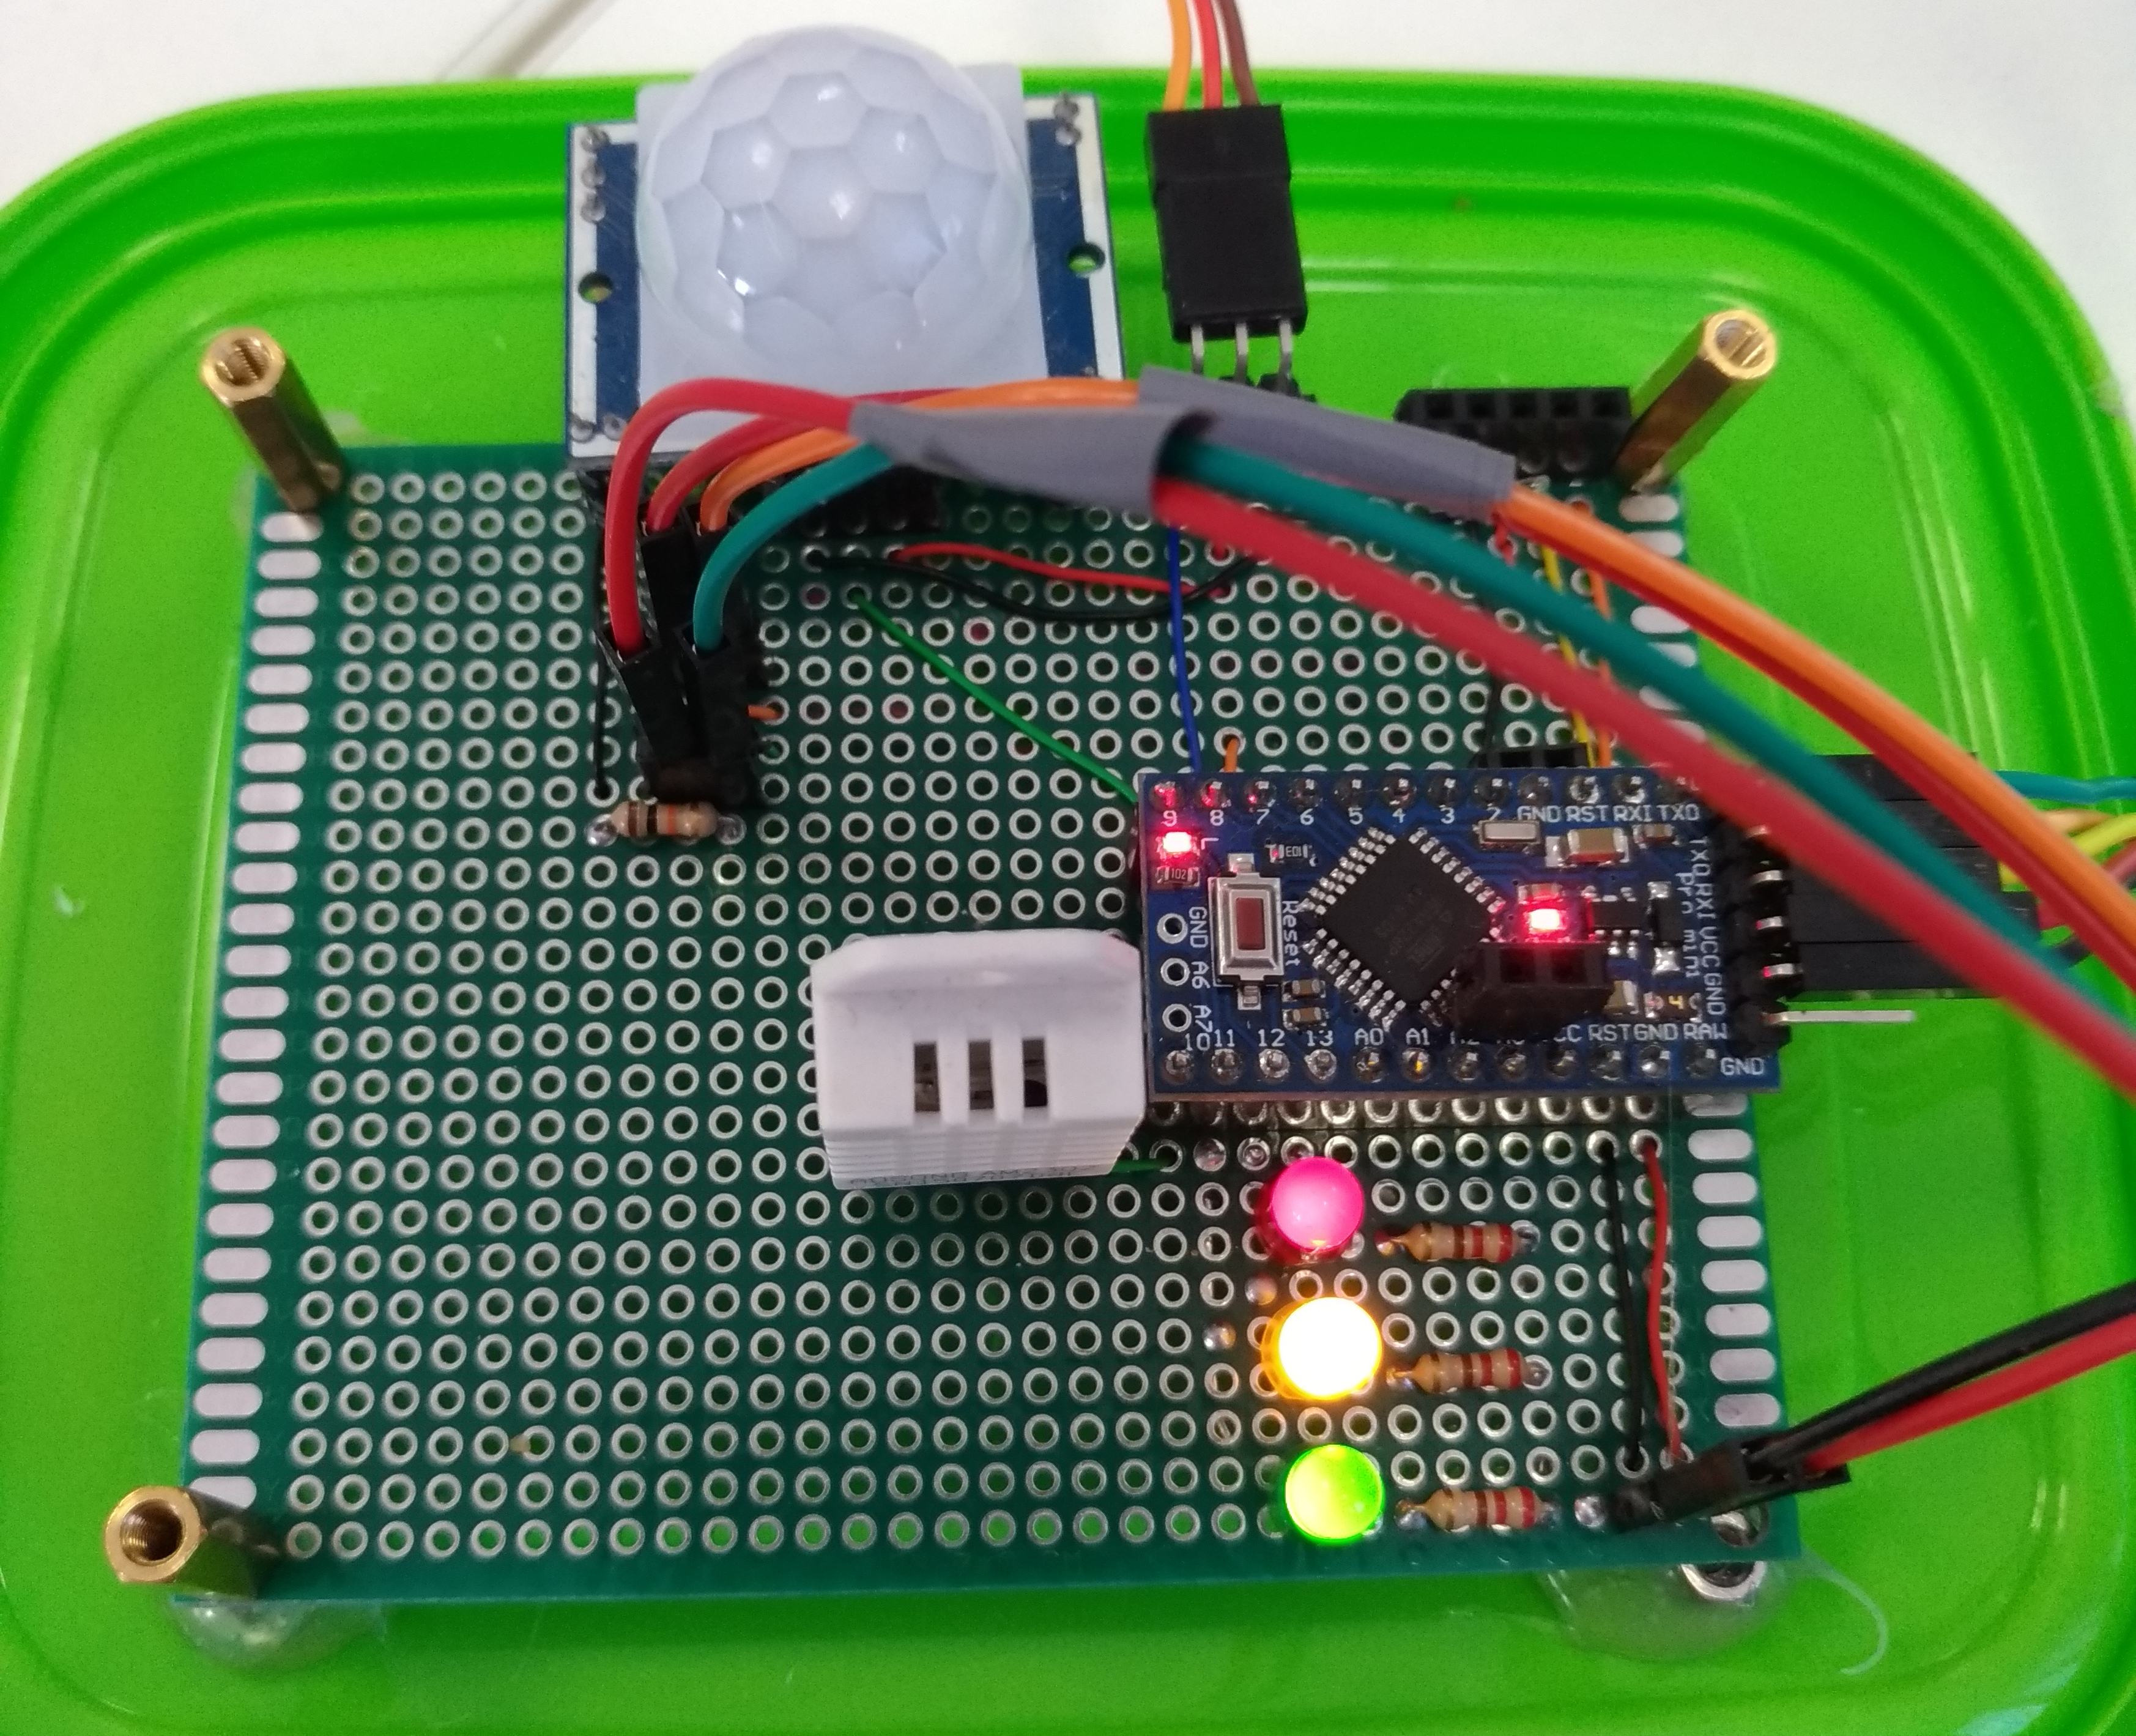
\includegraphics[width=4cm,keepaspectratio]{img/room_board}
		\caption{Room module}
		\label{fig:room_module}
		\end{subfigure}
	\vspace{1em} % here you can insert horizontal or vertical space
	\begin{subfigure}{0.4\textwidth} % width of right subfigure
		
\includegraphics[width=4cm,keepaspectratio]{img/valve}
		\caption{Valve}
		\label{fig:valve}
	\end{subfigure}
\end{figure}


The module is composed by:
\begin{itemize}
	\item Arduino pro mini, Atmega328P (8MHz, 3.3v logic)
	\item DHT22 Temperature and Humidity sensor
	\item PIR motion sensor
	\item Red led
	\item Green led
	\item Yellow led
	\item Servo Motor tower pro SG90
	\item 2 switch to check the open and closed position of the valve
\end{itemize}

\subsection{Components description}
\subsubsection{ServoMotor}
	\begin{figure}[h]
		\centering
		\begin{subfigure}{0.4\textwidth} % width of left subfigure
			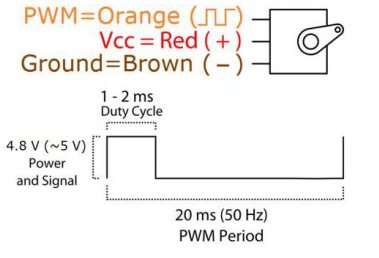
\includegraphics[width=4cm,keepaspectratio]{img/servo_signal}
			\end{subfigure}
		\vspace{1em} % here you can insert horizontal or vertical space
		\begin{subfigure}{0.4\textwidth} % width of right subfigure
			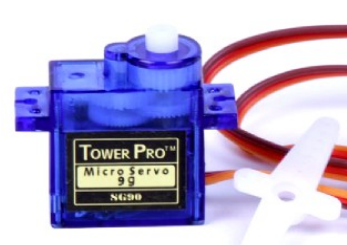
\includegraphics[width=4cm,keepaspectratio]{img/servomotor}
		\end{subfigure}
		\caption{Servo Motor}
		\label{fig:ServoMotor}
	\end{figure}

	The chosen Servo motor is a Tower Pro SG90 reported in \ref{fig:ServoMotor},
	As reported in the \ref{fig:ServoMotor}, the signal used to move the servomotor in the correct position is a PWM and the duty-cycle describe the position that the motor has to maintain.
	The signal to control the motor position is managed by the Servo library using the \textbf{timer1} a 16-bit timer.
	The digital circuit inside the servomotor will adjust the position of the rotor using a potentiometer attached to that.
	In the following table are reported	the characteristics of the servomotor:
	\begin{center}
		\begin{tabular}{||l | l | l||} 
			\hline
			Voltage(V) & 4.8 - 6 \\ 
			\hline
			Torque(Kg-cm) & 2.5 \\
			\hline
			Speed(sec) & 0.1 \\
			\hline
			Weight(g) & 14.7 \\
			\hline
		\end{tabular}
		\captionof{table}{Servo motor characteristics \label{tab:ServoCharacteristics}}
	\end{center}

\subsubsection{Valve position switches}
\begin{figure}[h]
	\centering
	
\includegraphics[width=6cm,keepaspectratio]{img/valve}
	\caption{Discovery board wiring}
	\label{fig:valve}
\end{figure}
In order to check the position of the valve, two switches are fixed in the open and closed position, during the \textit{valve initialization phase} the possible positions are computed starting from the open and closed position.
Whenever the valve is in the open or closed position a check is done using the switches.

\subsubsection{Temperature-Humidity Sensor}
The sensor DHT22 have been used for the project, in the following tables are reported the features of the sensors.
The sensor has a dedicated one-wire communication protocol implemented by the DHT adafruit library, a pull-up resistor is used in order to maintain the line clear when no one is transmitting.

\begin{center}
	\begin{tabular}{||l | l||} 
		\hline
		Voltage(V) & 3 - 5 \\ 
		\hline
		Current(mA) & 2.5 \\
		\hline
		Humidity(\%) & 0 - 100 \\
		\hline
		Humidity Accuracy(\%) & 2 - 5 \\
		\hline
		Temperature(C\degree) & -40 - 80 \\
		\hline
		Temperature Accuracy(C\degree) & +/- 0.5 \\
		\hline
		Sampling rate(Hz) & 0.5 \\
		\hline
	\end{tabular}
	\captionof{table}{DHT22 characteristics \label{tab:DHT22Characteristics}}
\end{center}


\subsection{Wiring}
	\begin{figure}[h]
		\centering
		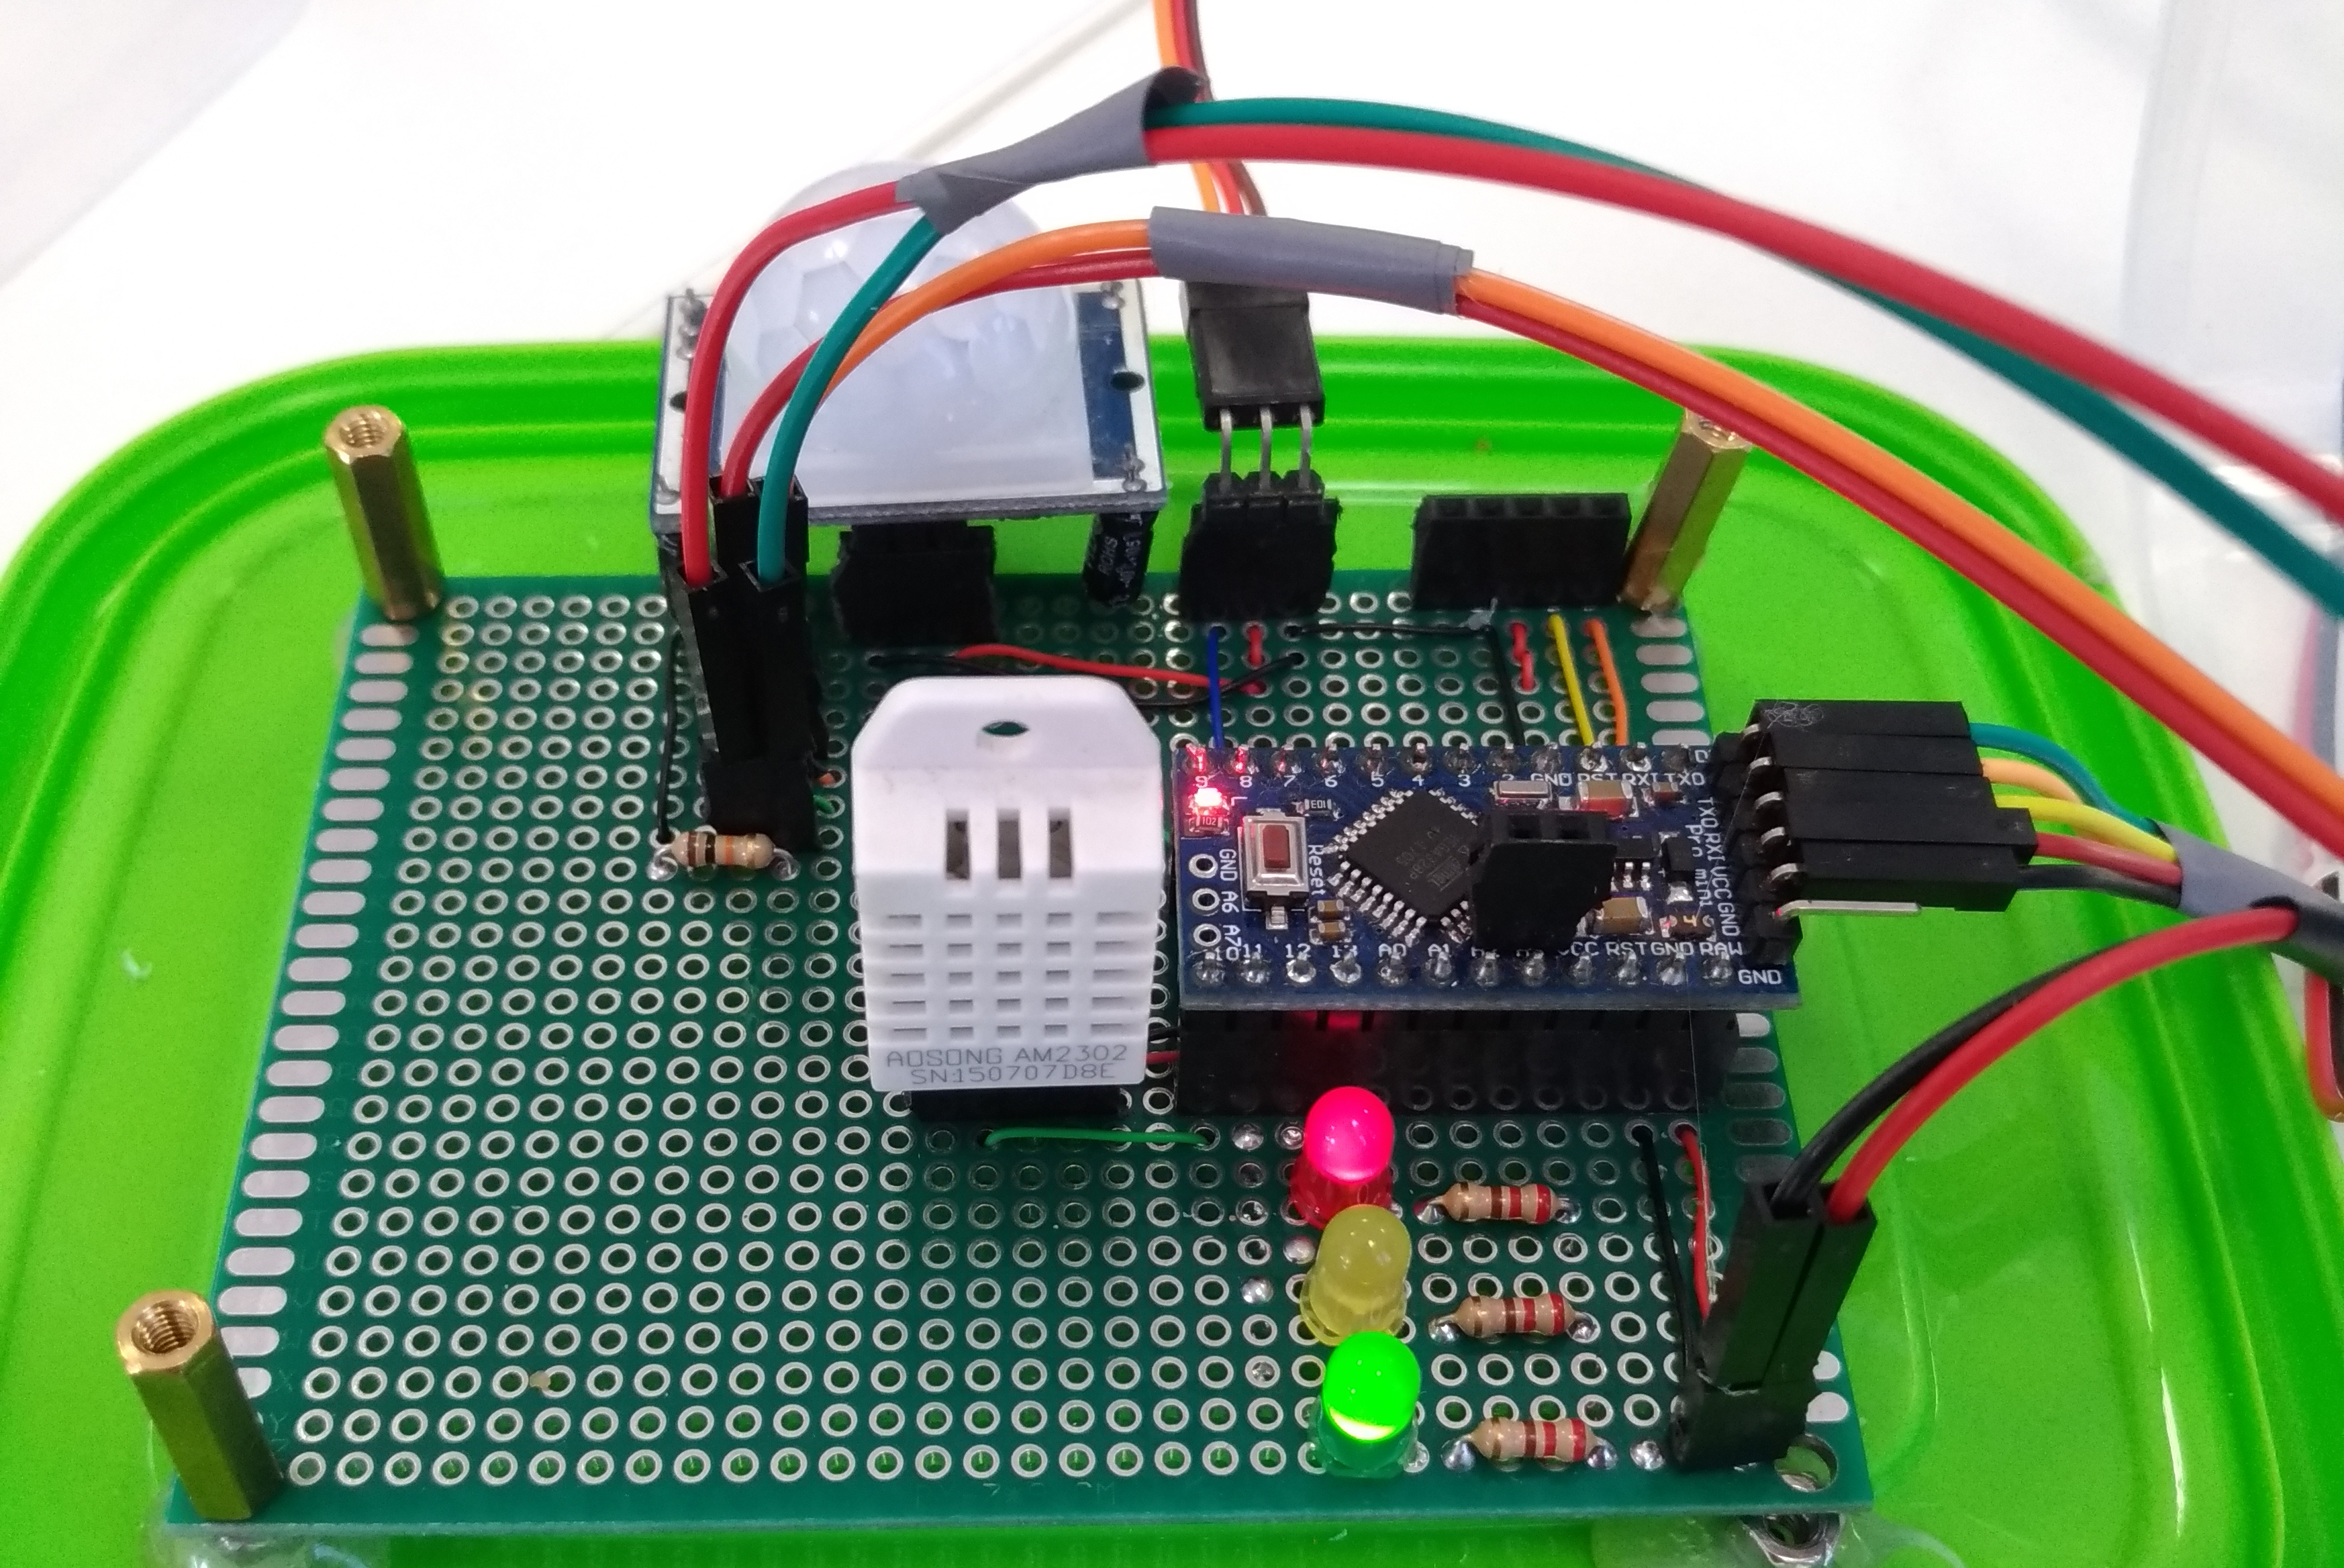
\includegraphics[width=6cm,keepaspectratio]{img/room_board_wiring}
		\caption{Room board wiring}
		\label{fig:room_wiring}
	\end{figure}
	The board is powered by 5V external power attached to the \textit{Raw pin}, this source is shared with the servomotor and the PIR sensor.
	In \ref{fig:room_wiring} is reported a picture of the implementation, in the following table the pins' configuration.
	\begin{center}
		\begin{tabular}{||l | l | l ||} 
			\hline
			Red led 			& 13 & D OUTPUT\\ 
			\hline
			Yellow led 			& 12 & D OUTPUT\\
			\hline
			Green data 			& 11 & D OUTPUT\\ 
			\hline
			DHT data 			& 10 & D INPUT\\ 
			\hline
			PIR data 			& 9 & D INPUT\\ 
			\hline
			ServoMotor PWM 		& 8 & D OUTPUT\\ 
			\hline
			Open Switch 		& 7 & D INPUT\\ 
			\hline
			Closed Switch 		& 6 & D INPUT\\ 
			\hline
			USART TX	 		& 0 & D OUTPUT\\ 
			\hline
			USART RX 			& 1 & D INPUT\\ 
			\hline
		\end{tabular}
		\captionof{table}{Atmega328P Wiring \label{tab:Atmega328Pwiring}}
	\end{center}
	
\section{JSON messages implementation}
As described in the SySML internal model of the system \ref{fig:CentralUnit_internals}, the modules exchange informations as \textit{RoomRequest} and \textit{RoomStatus}.
These messages have been implemented using the \textit{JSON} format, in the following are reported two messages exchanged during execution.
In the following version of the project the field names and the order of the variables must follow this example otherwise the simple JSON parser will consider the message as corrupted.

\subsection{Request Message}
\lstset{style=custompython}
\begin{lstlisting}[language=XML]
	{
		"Id":"01",
		"DTemp":"30.00"
	}
\end{lstlisting}

\subsection{Status Message}
\lstset{style=custompython}
\begin{lstlisting}[language=XML]
{
	"Id":"02","Eco":"0",
	"sens":[
		{"Nm":"Tmp","Val":"23.70","Fmt":"C"},
		{"Nm":"Hum","Val":"051.90","Fmt":"\%"}
	],
	"acts":[
		{"Nm":"Vlv","Val":"100","Fmt":"\%"}
	]
}
\end{lstlisting}
\newpage
\section{CUnit tests and simulation of the system}
In order to check the behaviour of the system a sequence of tests have been executed on the \textit{ESTA\_JSON\_lib} functions, that is used to convert the incoming JSON string from the module \textit{Room}.

\subsection{Variables tests}
For each variable present in the JSON message a boundary test is exeuted.
\newline
\begin{center}
	\begin{tabular}{|| c | c | c | c | c | c | c | c | c | c | c||} 
		\hline
		Variable				& 	Min 	& Max 	& 1\degree	& 2\degree & 3\degree	& 4\degree & 5\degree	& 6\degree & 7\degree\\ 
		\hline
		\textbf{Id}				&	1 		& 2		& 0 	& 1 	& 2 	& 3 	& / 	& / 	& / \\ 
		\hline
		\textbf{Eco}			&	0 		& 1		& -1  	& 0 	& 1 	& 2 	& / 	& /		& / \\ 
		\hline
		\textbf{Temperature}	&	15.0 	& 30.0	& 14.99 & 15.0 	& 15.01 & 29.99	& 30.00 & 30.01 & 22.5 \\ 
		\hline
		\textbf{Humidity}		&	0.0		& 100.0	& -0.01	& 0.0 	& 0.01 	& 99.99 & 100.00 & 100.01 & 50.00 \\ 
		\hline
		\textbf{Valve}			&	0		& 100 	& -1 	& 0 	& 1 	& 99 	& 100 	& 101 	& 50 \\ 
		\hline
	\end{tabular}
	\captionof{table}{Variables tests \label{tab:VariablesTests}}
\end{center}

\subsection{JSON Compliance  tests}
In order to check the \textit{JSON compliance code checker} the following tests are applied modifying a correct message.
\begin{center}
	\begin{tabular}{||c | c ||} 
		\hline
		Number			& 	Description \\ 
		\hline
		\textbf{1}		&	Missing odd number of \textit{\{}\\ 
		\hline
		\textbf{2}		&	Missing odd number of \textit{"}\\ 
		\hline
		\textbf{3}		&	Missing odd number of \textit{[}\\ 
		\hline
		\textbf{4}		&	Check field name \textit{Id} \\ 
		\hline
		\textbf{5}		&	Check field name \textit{Eco} \\ 
		\hline
		\textbf{6}		&	Check field name \textit{Nm} \\ 
		\hline
		\textbf{7}		&	Check field name \textit{Val} \\ 
		\hline
		\textbf{8}		&	Check field name \textit{Fmt} \\ 
		\hline
		\textbf{9}		&	Check field name \textit{Tmp} \\ 
		\hline
		\textbf{10}		&	Check field name \textit{Hum} \\ 
		\hline
		\textbf{11}		&	Check field name \textit{Vlv} \\ 
		\hline
		\textbf{12}		&	Check Temperature format value \textit{C} \\ 
		\hline
		\textbf{13}		&	Check Humidity format value \textit{\%} \\ 
		\hline
		\textbf{14}		&	Check Valve format value \textit{\%} \\ 
		\hline
	\end{tabular}
	\captionof{table}{JSON compliance tests \label{tab:JSONComplianceTests}}
\end{center}

In the following picture \ref{fig:CUnit_result} is reported the result of the tests executed using the framework \textit{CUnit} Version 2.1.3.
\begin{figure}[H]
	\centering
	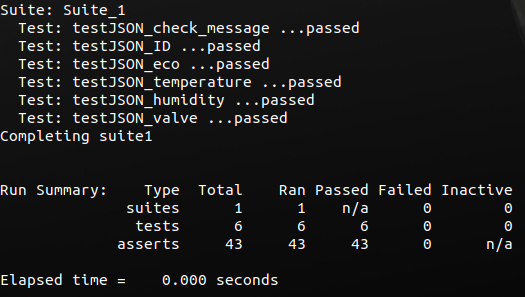
\includegraphics[width=8cm,keepaspectratio]{img/CUnit_result}
	\caption{CUnit results}
	\label{fig:CUnit_result}
\end{figure}


\subsection{Network noise tests}
In order to check the correctness behaviour of the \textit{Central Unit} module a python script that simulates the rooms has been created and used to test the module simulating two different rooms.
The \textbf{Room simulator} creates the correct JSON string and send it, in order to simulate the \textbf{noise} of the network this cases have been considered:
\begin{center}
	\begin{tabular}{||c | c | c ||} 
		\hline
		Number			& 	Description & Probability\\ 
		\hline
		\textbf{1}		&	Message lost, the response message is discarded & 0.1 \\ 
		\hline
		\textbf{2}		&	Message corrupted, 3 random characters are replaced with \textit{?} & 0.1\\ 
		\hline
	\end{tabular}
	\captionof{table}{Network noise tests \label{tab:NetworkNoiseTests}}
\end{center}
\begin{figure}[H]
	\centering
	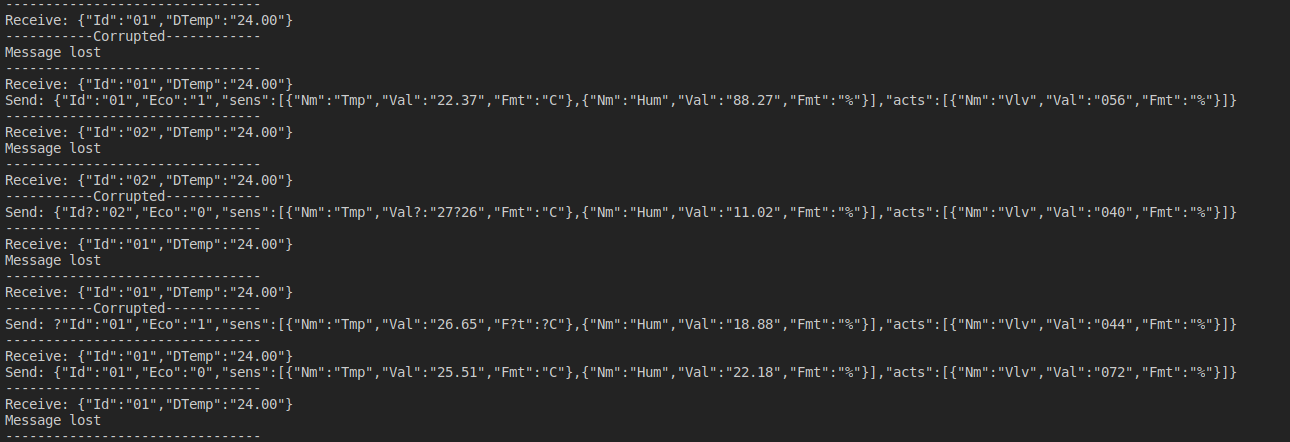
\includegraphics[width=12cm,keepaspectratio]{img/room_simulator}
	\caption{Room simulator}
	\label{fig:roomsimulator}
\end{figure}
\begin{thebibliography}{9}
	\bibitem{moveit} 
\end{thebibliography}

\end{document}